\documentclass[12pt,letterpaper]{ryerson}

% fix the colors of dept_sales figure.
% fix scaling of state_sales figure.

% LSTM
%% Results
\newcommand\lstmTrnME{0.02139}
\newcommand\lstmValME{-0.00857}
\newcommand\lstmTstME{-0.10333}
\newcommand\lstmTstMonME{-0.10991}

\newcommand\lstmTrnRMSE{2.10657}
\newcommand\lstmValRMSE{2.11495}
\newcommand\lstmTstRMSE{2.24916}
\newcommand\lstmTstMonRMSE{2.27780}

\newcommand\lstmTrnRMSSE{0.78320}
\newcommand\lstmValRMSSE{0.82372}
\newcommand\lstmTstRMSSE{0.85677}
\newcommand\lstmTstMonRMSSE{0.80511}

%% Hyperparameters
\newcommand\lstmParamsNlayers{3}
\newcommand\lstmParamsNunits{405}
\newcommand\lstmParamsScale{0.752032}
\newcommand\lstmParamsLR{0.000534}
\newcommand\lstmParamsDecay{0.000445}
\newcommand\lstmParamsDropout{0.225848}
\newcommand\lstmParamsNorm{0}
\newcommand\lstmParamsBatch{59}
\newcommand\lstmParamsSteps{23}

\newcommand\lstmParamsRangeNlayers{Integer(3, 5)}
\newcommand\lstmParamsRangeNunits{Integer(128, 512)}
\newcommand\lstmParamsRangeScale{Float(0.2, 1)}
\newcommand\lstmParamsRangeLR{Float(0.0001, 0.01)}
\newcommand\lstmParamsRangeDecay{Float(0, 0.001)}
\newcommand\lstmParamsRangeDropout{Float(0, 0.3)}
\newcommand\lstmParamsRangeNorm{Integer(0, 1)}
\newcommand\lstmParamsRangeBatch{Float(32, 128)}
\newcommand\lstmParamsRangeSteps{Integer(14, 56)}

% MLP
%% Results
\newcommand\annTrnME{-0.05645}
\newcommand\annValME{-0.03643}
\newcommand\annTstME{-0.08568}
\newcommand\annTstMonME{\annTstME}

\newcommand\annTrnRMSE{2.73888}
\newcommand\annValRMSE{2.24467}
\newcommand\annTstRMSE{2.29376}
\newcommand\annTstMonRMSE{\annTstRMSE}

\newcommand\annTrnRMSSE{0.94049}
\newcommand\annValRMSSE{0.87421}
\newcommand\annTstRMSSE{0.87376}
\newcommand\annTstMonRMSSE{0.81075}

%% Hyperparameters
\newcommand\annParamsNlayers{4}
\newcommand\annParamsNunits{467}
\newcommand\annParamsScale{0.699088}
\newcommand\annParamsLR{0.004514}
\newcommand\annParamsDecay{0.000478}
\newcommand\annParamsDropout{0.006266}
\newcommand\annParamsNorm{0}
\newcommand\annParamsBatch{57798}

\newcommand\annParamsRangeNlayers{Integer(3, 5)}
\newcommand\annParamsRangeNunits{Integer(64, 512)}
\newcommand\annParamsRangeScale{Float(0.2, 1)}
\newcommand\annParamsRangeLR{Float(0.0001, 0.01)}
\newcommand\annParamsRangeDecay{Float(0, 0.001)}
\newcommand\annParamsRangeDropout{Float(0, 0.3)}
\newcommand\annParamsRangeNorm{Integer(0, 1)}
\newcommand\annParamsRangeBatch{Float(32000, 100000)}

% LGBM
%% Results
\newcommand\lgbmTrnME{-0.00001}
\newcommand\lgbmValME{-0.00679}
\newcommand\lgbmTstME{-0.07056}
\newcommand\lgbmTstMonME{\lgbmTstME}

\newcommand\lgbmTrnRMSE{2.34224}
\newcommand\lgbmValRMSE{2.11933}
\newcommand\lgbmTstRMSE{2.18648}
\newcommand\lgbmTstMonRMSE{\lgbmTstRMSE}

\newcommand\lgbmTrnRMSSE{0.80429}
\newcommand\lgbmValRMSSE{0.82540}
\newcommand\lgbmTstRMSSE{0.83289}
\newcommand\lgbmTstMonRMSSE{0.77283}

%% Hyperparameters
\newcommand\lgbmParamsLR{0.097892}
\newcommand\lgbmParamsFeatFrac{0.553332}
\newcommand\lgbmParamsLambda{0.219554}
\newcommand\lgbmParamsNleaves{749}
\newcommand\lgbmParamsMinData{1534}

\newcommand\lgbmParamsRangeLR{Float(0.001, 0.5)}
\newcommand\lgbmParamsRangeFeatFrac{Float(0.2, 1)}
\newcommand\lgbmParamsRangeLambda{Float(0, 0.3)}
\newcommand\lgbmParamsRangeNleaves{Integer(50, 5000)}
\newcommand\lgbmParamsRangeMinData{Integer(10, 5000)}

% Hybrid
%% Results
\newcommand\hybTrnME{0.01417}
\newcommand\hybValME{-0.04265}
\newcommand\hybTstME{-0.14021}
\newcommand\hybTstMonME{-0.11916}

\newcommand\hybTrnRMSE{2.10155}
\newcommand\hybValRMSE{2.11706}
\newcommand\hybTstRMSE{2.26268}
\newcommand\hybTstMonRMSE{2.25698}

\newcommand\hybTrnRMSSE{0.78133}
\newcommand\hybValRMSSE{0.82453}
\newcommand\hybTstRMSSE{0.86192}
\newcommand\hybTstMonRMSSE{0.79775}
\interdisplaylinepenalty = 2500


\usepackage[inline]{enumitem}
\PassOptionsToPackage{hyphens}{url}
\usepackage{hyperref} 
\usepackage{graphicx}
\usepackage{array, makecell}
\usepackage{wrapfig}
\usepackage{setspace}
\usepackage[page]{appendix}
\usepackage{blindtext}
\usepackage[font=small,labelfont=bf,skip=5pt]{caption}
\usepackage{charter}
\usepackage{float}
\input{insbox.tex}
\usepackage{titlesec}
\usepackage{apptools}

\titleformat{\chapter}[display]{\normalfont\huge\bfseries}{\chaptertitlename\ \thechapter}{20pt}{\Huge}   
\titlespacing*{\chapter}{0pt}{-10pt}{25pt}

\renewcommand{\ttdefault}{Computer Modern}
\newcommand\Tstrut{\rule{0pt}{2.6ex}}         % = `top' strut
\newcommand\Bstrut{\rule[-0.9ex]{0pt}{0pt}}   % = `bottom' strut


\setAuthor{Moeen Bagheri}
\setTitle{\textbf{Walmart Multi-Step Sales Forecasting}}
\setThesisDegree{Master of Science (MSc)}
\setUniversity{Ryerson University}
\setDepartment{Data Science and Analytics}
\setLocation{Toronto, Ontario, Canada}
\setThesisYear{2020}

\setAuthorsDeclaration{
I hereby declare that I am the sole author of this MRP. This is a true copy of the MRP, including any required final revisions. \newline

\noindent I authorize Ryerson University to lend this MRP to other institutions or individuals for the purpose of scholarly research. \newline

\noindent I further authorize Ryerson University to reproduce this MRP by photocopying or by other means, in total or in part, at the request of other institutions or individuals for the purpose of scholarly research. \newline

\noindent I understand that my MRP may be made electronically available to the public. \newline

\noindent Moeen Bagheri
}

\setAbstract{
Forecasting future sales is important to retailers for managing inventory and making marketing decisions. 
Product sales are affected by many external factors, which must be considered when forecasting future sales.
In this paper, the effects of these factors were directly taken into account in the four models created.
These four models include three singular models, consisting of LSTM, MLP, and LGBM, as well as a hybrid model.
The hyperparameters of the singular models were optimized using Bayesian optimization.
Furthermore, we aimed to provide 28-days ahead sale forecasts, by forecasting one day at a time.
The LGBM model was able to achieve the best performance, followed by the hybrid model.
The outstanding results of the LGBM model shows the potential of boosting methods in improving the overall performance.
Moreover, the LSTM model was able to outperform the MLP model, which demonstrates the ability of LSTM networks in learning from time-series data. \newline

\noindent\keywords{
    Retail, 
    Forecasting, 
    Long Short-Term Memory, 
    Multilayer Perceptron,
    Hybrid, 
    LightGBM, 
    Bayesian Optimization
}
}
\setAcknowledgements{I am very thankful of \textbf{Dr. Konstantinos Georgiou} for his continuous support and assistance during the semester. Dr. Georgiou provided me with valuable feedback and helped me with thinking critically about the problem. He also provided valuable comments regarding the structure and contents of the paper. I am grateful to Dr. Georgiou for making this project a reality.
}


\begin{document}

\begin{ryerson}
\chapter{Introduction}
Sales forecasting is crucial for retailers in order to predict the future demand of products, which can in turn increase profit by ensuring the replenishment of the necessary supply to meet future demand, as well as minimizing product waste \cite{c13}.
However, the volatility in demand makes sales forecasting a challenging problem \cite{c14}.
This volatility is dependent on many external factors, such as holidays, events, price, and promotions.
Hence, it is necessary to take into account the effects of these external factors when forecasting future sales.
In some approaches, the manager guides the forecasting model based on his/her knowledge of the external factors by using fuzzy logic.
However, recent studies have focused on creating models that are able to directly take into account the effects of these external factors.
Moreover, most retail stores contain multiple sale channels and require sale forecasts longer than one day ahead in the future, which adds another level of complexity to the problem.

In this paper, we will compare the performance of three models, which consist of Long Short-Term Memory (LSTM), Multi-Layer Perceptron (MLP), and LightGBM (LGBM) models, in forecasting 28 days ahead in the future.
Additionally, the LSTM model and the best performing model between the MLP and LGBM models will be used to construct a hybrid model to check if it is able to improve the performance compared to the two singular models.
Furthermore, the hyperparameters of all models will be optimized using Bayesian optimization.

\chapter{Literature Review}
Numerous statistical and deep learning methods have been employed in the past for forecasting sales.
Linear statistical models, such as multivariate linear regression, which make predictions based on the historical relationship between different influential factors and the demand, have the advantage of being efficient. 
However, these linear models perform well for linear problems, where the relationship between the dependent variable and one or more independent variables is linear with a constant rate of change, and hence fail to capture the nonlinear relationships and describe the complexity of the supply chain \cite{c5}.
Similarly, basic univariate models, such as ARIMA, which consider the data as a time-series, are also unable to describe the complexity of the supply chain since they are only capable of capturing linear relationships in the data \cite{c5, c1}.
On the other hand, nonlinear statistical models used for sales forecasting include Bayesian networks, support vector machines, and Markov chains. 
Unlike linear models, these models are able to learn complex nonlinear relationships from the data.
In a study done in \cite{c10}, a Random Forest model was used to forecast Major League Baseball game ticket sales.
Their approach consisted of a dynamic month-ahead forecasting strategy, where the data is updated every month. 
Their results showed that their proposed RF model slightly outperforms their baseline model, which they chose to be an Ordinary Least Squares (OLS) regression model.
However, even though nonlinear statistical models have a high capability of solving complex problems, selecting the right model for a certain problem is a difficult task, which requires expert knowledge of statistical models. 
Moreover, these methods are usually found to perform worse compared to deep learning methods \cite{c5}. 

Deep learning methods are able to automatically extract important features and have been found to obtain better results compared to statistical models \cite{c5}. 
The self-organizing and self-adjusting capabilities of Artificial Neural Networks (ANN) allows them to solve complex nonlinear problems \cite{c7}.  
In a study done by \cite{c9}, a Multi-Layer Perceptron (MLP) was used to predict the monthly sale volumes of a Polish company, which imports fabric on a monthly basis, based on the previous three months.
The MLP contained three input neurons, a single hidden layer with 15 neurons, as well as one output neuron, and was able to achieve a high accuracy on the data with a Root-Mean-Square Error (RMSE) of 3.34e-11.
However, even though ANNs excel at solving complex problems, they lack the ability to interpolate and predict long-term sequences \cite{c7}.
Alternatively, deep learning methods, such as LSTM, are able to preserve past information and capture the temporal relationships in the data \cite{c6}.
However, even though deep learning methods can improve the accuracy of the predictions compared to statistical models, it is much more challenging to interpolate and draw conclusions from their results \cite{c5, c9}. 

In a study done in \cite{c11}, the performances of ARIMA, MLP, and LSTM models were compared for forecasting and predicting cash flow.
Interest Opportunity Cost (IOC), which is a measure based on financial concepts and allows finance-specific comparison of the models, was used in MLP and LSTM as the error function to be optimized.
According to their results, LSTM was able to obtain the minimum error of 0.09, compared to MLP and ARIMA with an error of 0.10 and 0.23, respectively.
The cash flow data exhibited a strong weekly pattern that assisted LSTM in its predictions. 
However, due to the small amount of data available (3 years), variances caused by holidays and other special events could not be explained.

On a separate note, many methods do not take into account external variables and factors, such as price changes and promotions and have been shown to only perform well in periods without the influence of any external factors \cite{c2, c3}. 
In practice, in order to incorporate the effects of promotions on the sales, many retailers use a base-times-lift approach, where the sales are first forecasted based on a simple time-series and then adjusted based on the incoming promotions \cite{c4}. 
Recent studies have focused on optimizing these adjustments, which are made based on promotions and other external factors \cite{c4}. 
In an alternative approach, hybrid models have been used in order to take advantage of the strengths of different models together, which helps capture both the temporal information in the data, as well as the correlation between the demand and the external factors \cite{c5, c8}. 
The complex behaviour of a time-series cannot be explained by a single model if, for example, the time-series contains both linear and nonlinear correlations \cite{c12}.
Hybrid models are usually constructed in a sequential manner, where the first component is fitted to the data first, and then the second component is fitted to the residuals of the first component \cite{c12}.
The residuals of a model contain the information that could not be captured by that model \cite{c8}.
However, hybrid models are not guaranteed to perform better than single models and model selection is still a crucial aspect of hybrid models \cite{c12}.

The study done by \cite{c8} presents an example of a hybrid model used for forecasting. 
In this study, an LSTM model is combined with a Random Forest model to create a hybrid model for forecasting sales of a store with one online and 11 offline sale channels.
In the hybrid model, LSTM is applied first to capture the linear and non-linear temporal information from the data. 
Next, the residuals from the LSTM are used as the dependant variable and the external variables are used as the independent variable in a Random Forest model in order to capture the non-temporal relationships in the data. 
Another challenge to address is the modeling of sales across multiple channels. 
One approach would be to model each channel separately, however, this approach will eliminate the aggregate demand information from the data. 
Therefore, this study forecasted the demand of a product based on its order origin (online vs. offline) instead in order to sustain the aggregate demand information.
Their results showed that the hybrid model performed better than its two components, LSTM and RF, individually. 


\chapter{Exploratory Data Analysis}
The dataset \cite{dataset} includes the unit sales of 3,049 products sold by Walmart in the USA in grouped time-series format. 
The products are classified in three categories (Hobbies, Foods, and Household) and seven departments. 
Additionally, these products are sold across ten stores, located in the three states of California (CA), Texas (TX), and Wisconsin (WI). Specifically, there are four stores located in California, three in Texas, and three in Wisconsin.
The dataset contains the following three data files \cite{m5}:
\begin{itemize}
    \item \textbf{calendar.csv}: contains information about the dates the products were sold, such as promotions, holidays, and other events.
    \item \textbf{sell\_prices.csv}: contains the average weekly price of each item.
    \item \textbf{sales\_train.csv}: contains the daily unit sales of each item.
\end{itemize}

\begin{wrapfigure}{r}{0.46\textwidth}
    \vspace{-25pt}
    \centering
    \captionsetup{width=.46\textwidth}
    \fbox{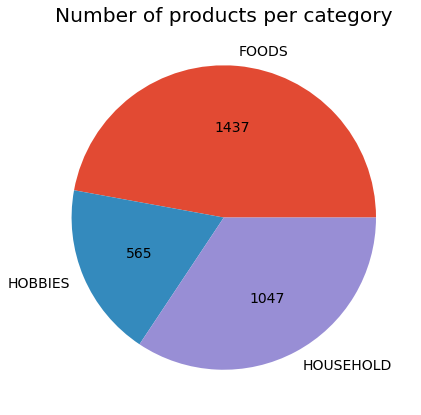
\includegraphics[width=0.42\textwidth]{figures/exploratory_data_analysis/item_cats.png}}
    \caption{Number of products per category.}
    \label{fig:item_cats}
    \vspace{-20pt}
\end{wrapfigure}

Figure \ref{fig:item_cats} shows the number of products per category. 
There are 1437, 1047, and 565 products in the \texttt{Foods}, \texttt{Household}, and \texttt{Hobbies} categories, respectively, for a total of 3049 products. 
Since these products are sold across ten different stores, there is a total of 30,490 items, out of which 22,243 had a price change at some point in time. 
In addition, from Figure \ref{fig:price_all}, which shows the price distribution of all products, we can see that most items cost between three to four dollars.
Furthermore, Figure \ref{fig:price_cats} shows the price distribution of each product category separately.
It is apparent that the \texttt{Hobbies} products do not have the same price distribution as \texttt{Foods} and \texttt{Household} products and tend to have more products that are very cheap.

\begin{figure}[b!]
    \centering
    \captionsetup{width=.93\textwidth}
    \fbox{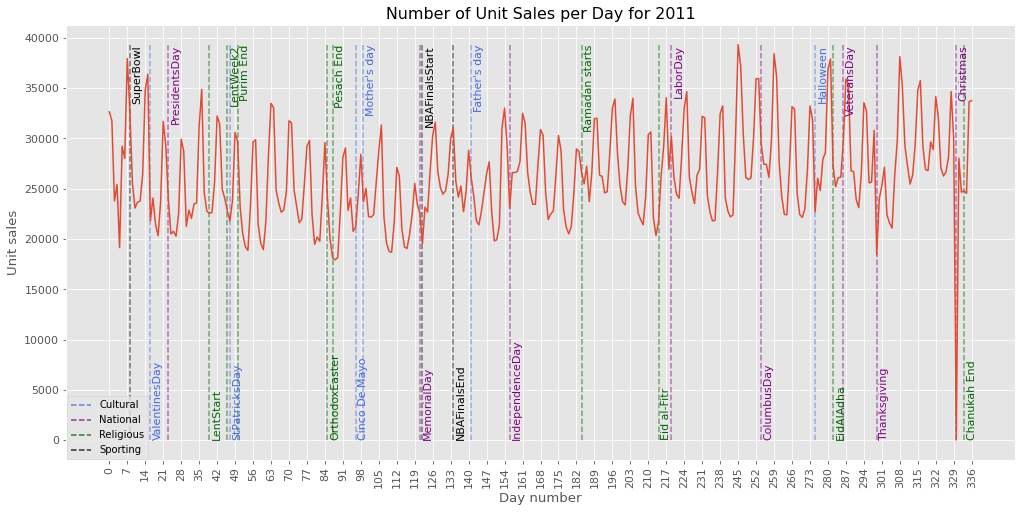
\includegraphics[width=0.93\textwidth]{figures/exploratory_data_analysis/daily_sales_2011.png}}
    \caption{The number of unit sales per day in 2011.}
    \label{fig:daily_sales_2011}
\end{figure}

\begin{figure}[t]
    \centering
    \captionsetup{width=.93\textwidth}
    \fbox{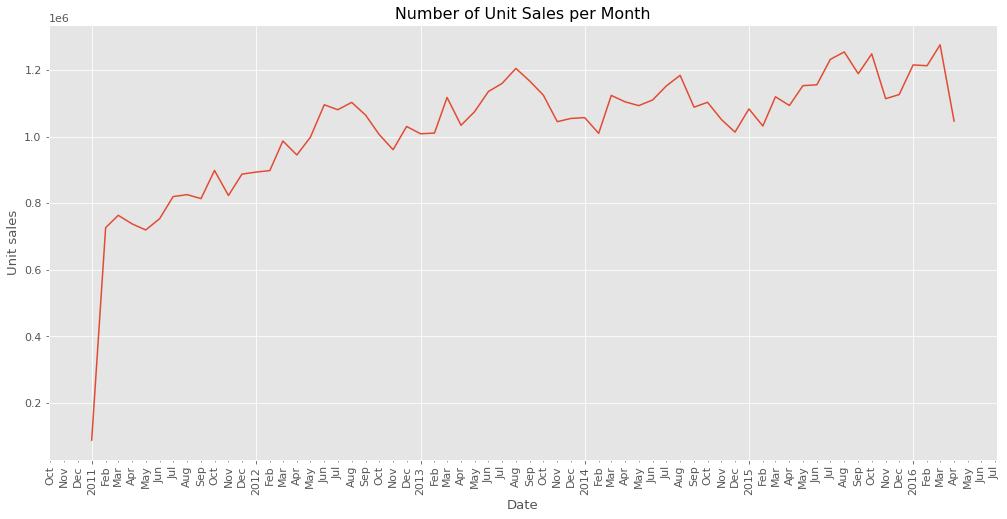
\includegraphics[width=0.93\textwidth]{figures/exploratory_data_analysis/monthly_sales.png}}
    \caption{The number of unit sales per month.}
    \label{fig:monthly_sales}
    \vspace{-2.5mm}
\end{figure}

On another point, Figure \ref{fig:ma_4week} shows a 4-week moving-average of the revenue earned, number of units sold, and the average price of all items.
We see that the average price of products are increasing over time in a linear fashion. Moreover, as expected, revenue and unit sales have increased with almost an identical pattern. Additionally, examining the revenue and unit sales graphs, we can see some form of seasonality in the curves.
Hence, we further explore for any seasonality patterns. From Figure \ref{fig:daily_sales_2011}, which shows the number of unit sales per day for the year 2011, we see a clear weekly pattern in the number of unit sales.
Specifically, the number of units sold tends be the highest during the weekends and the lowest in the middle of the week. 
This can be confirmed by examining Figure \ref{fig:dow_sales}, which shows the average number of units sold per day of week for all years.
Additionally, Figure \ref{fig:daily_sales_2011} shows national holidays and other special events, which are considered as external factors and may affect the number of unit sales. 
Most national holiday events, such as Thanksgiving, have a negative effect on the number of unit sales, possibly because people tend to spend time with their families rather than shopping. 
Additionally, Figure \ref{fig:monthly_sales} shows the number of unit sales per month, which shows that the number of sales tend to increase as we approach the middle of the year and falls off at the end of the year.
Moreover, we can see a spike in sales during March.
This is confirmed by examining Figure \ref{fig:moy_sales}, which shows the average number of units sold in each month of the year. 

\begin{figure}[H]
    \begin{minipage}{0.48\textwidth}
        \centering
        \vspace{3mm}
        \captionsetup{width=.98\textwidth}
        \fbox{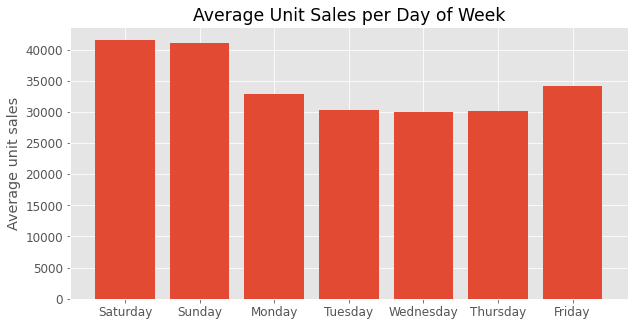
\includegraphics[width=0.98\textwidth]{figures/exploratory_data_analysis/dow_sales.png}}
        \caption{Average number of units sold per day of week.}
        \label{fig:dow_sales}
    \end{minipage}
    \hfill
    \begin{minipage}{0.48\textwidth}
        \centering
        \captionsetup{width=.98\textwidth}
        \fbox{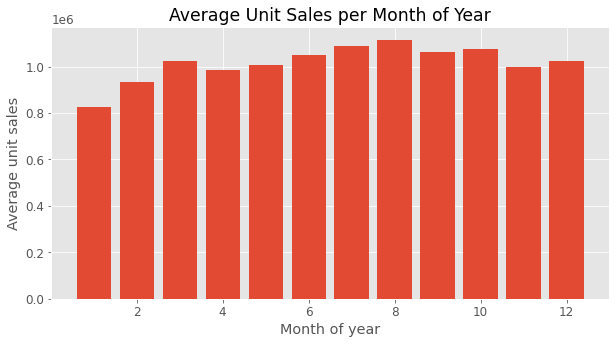
\includegraphics[width=0.98\textwidth]{figures/exploratory_data_analysis/moy_sales.png}}
        \caption{Average number of units sold per month.}
        \label{fig:moy_sales}
    \end{minipage}
\end{figure}

In the rest of this chapter, we will group the items based on their categories, states, stores, and departments and compare their sales data.

\begin{figure}[b!]
    \centering
    \captionsetup{width=0.98\textwidth}
    \fbox{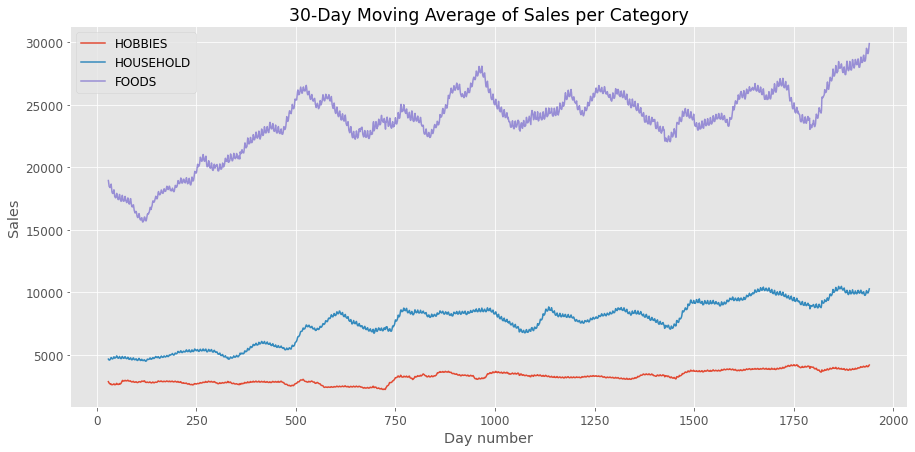
\includegraphics[width=0.98\textwidth]{figures/exploratory_data_analysis/cat_sales.png}}
    \caption{30-day moving average of sales per category.}
    \label{fig:cat_sales}
\end{figure} 

\section{Product Categories}
\begin{wrapfigure}{r}{0.55\textwidth}
    \vspace{-15pt}
    \centering
    \captionsetup{width=0.52\textwidth}
    \fbox{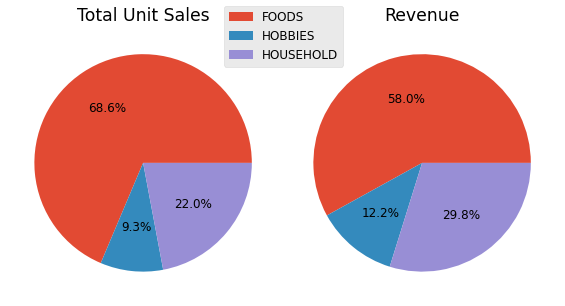
\includegraphics[width=0.52\textwidth]{figures/exploratory_data_analysis/sales_rev_cats.png}}
    \caption{Proportion of units sold and revenue earned in each product category.}
    \label{fig:sales_rev_cats}
    \vspace{-20pt}
\end{wrapfigure}
   
Furthermore, we examine the number of units sold and revenue earned from each product category.
By examining the pie charts in Figure \ref{fig:sales_rev_cats}, we see that the \texttt{Foods} category accounts for most of the units sold and revenue earned, with 68.6\% of all products sold belonging to the \texttt{Foods} category, which corresponds to 58.0\% of the total revenue earned.
Moreover, figure \ref{fig:cat_sales} shows a time-series of the number of unit sales per category.
It is apparent that the \texttt{Foods} category has a lot more sales that the other two categories.
Moreover, the sales for the \texttt{Foods} category seem to have a lot of oscillations that is less present in the other two categories.

\begin{figure}[b!]
    \centering
    \captionsetup{width=0.98\textwidth}
    \fbox{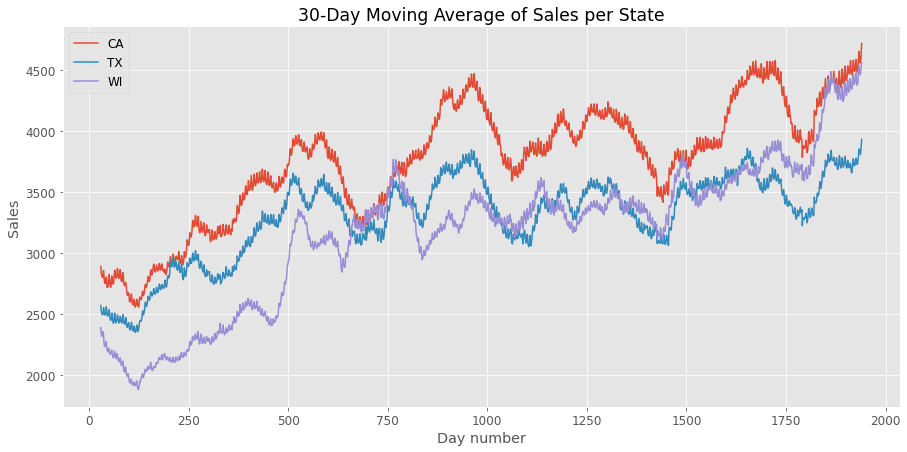
\includegraphics[width=0.98\textwidth]{figures/exploratory_data_analysis/state_sales.png}}
    \caption{30-day moving average of sales per category.}
    \label{fig:state_sales}
\end{figure} 

\section{States}
\begin{wrapfigure}{r}{0.55\textwidth}
    \vspace{-10pt}
    \centering
    \captionsetup{width=0.52\textwidth}
    \fbox{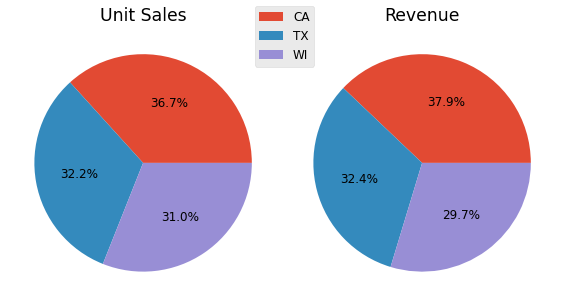
\includegraphics[width=0.52\textwidth]{figures/exploratory_data_analysis/sales_rev_states.png}}
    \caption{Proportion of units sold and revenue earned in each state.}
    \label{fig:sales_rev_states}
    \vspace{-20pt}
\end{wrapfigure}
Another factor to examine is whether there is any difference in the number of units sold and revenue earned between various states.
Figure \ref{fig:sales_rev_states} compares the total unit sales and revenue earned in each state. 
Since the number of stores is not constant between the states, the values for each state have been normalized by the number of stores in that state.
By examining the pie charts we see that, on average, the three states have about the same number of unit sales and revenue earned per store, however, the store in state of California are, on average, performing slightly better compared to the stores in Texas and Wisconsin. 
Furthermore, Figure \ref{fig:state_sales} shows that the state California has more oscillations in its sales compared to the other states.


\begin{figure}[b!]
    \centering
    \fbox{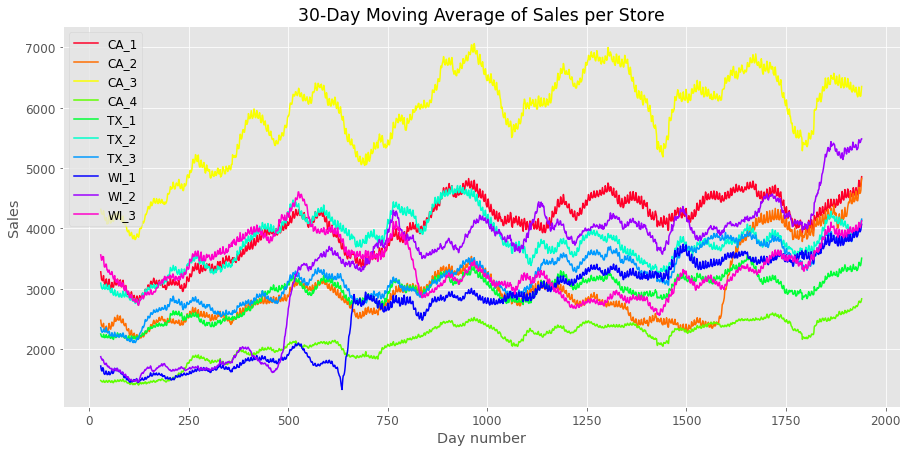
\includegraphics[width=0.98\textwidth]{figures/exploratory_data_analysis/store_sales.png}}
    \caption{30-day moving average of sales per store.}
    \label{fig:store_sales}
\end{figure} 

\section{Stores}
\begin{wrapfigure}{r}{0.55\textwidth}
    \vspace{-15pt}
    \centering
    \captionsetup{width=0.52\textwidth}
    \fbox{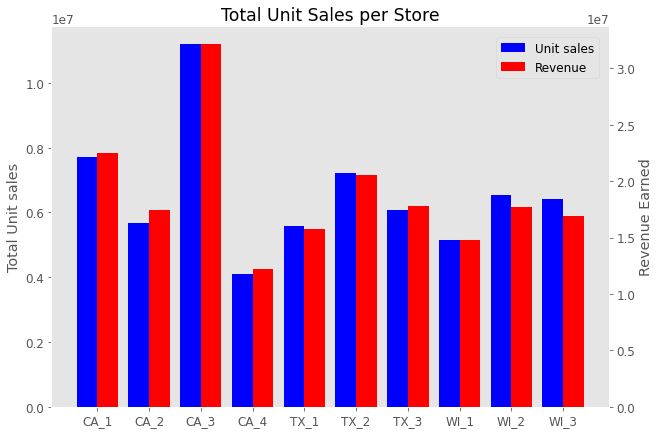
\includegraphics[width=0.52\textwidth]{figures/exploratory_data_analysis/sales_rev_stores.png}}
    \caption{Proportion of units sold and revenue earned per store.}
    \label{fig:sales_rev_stores}
    \vspace{-20pt}
\end{wrapfigure}
There are a total of nine stores in the dataset.
The bar chart in figure \ref{fig:sales_rev_stores} compares the number of unit sales and revenue earned between each stores.
From this figure, we can see that store \texttt{CA\_3} has the highest number of unit sales and revenue earned, and store \texttt{CA\_4} has the lowest number of unit sales and revenue earned.
We can further confirm this by examining the time-series of the number of sales per store, shown in Figure \ref{fig:store_sales}.
Moreover, this figure shows that store \texttt{CA\_3} has a lot more volatility in its sales than the other stores.

\section{Departments}
\begin{wrapfigure}{r}{0.55\textwidth}
    \vspace{-10pt}
    \centering
    \captionsetup{width=0.52\textwidth}
    \fbox{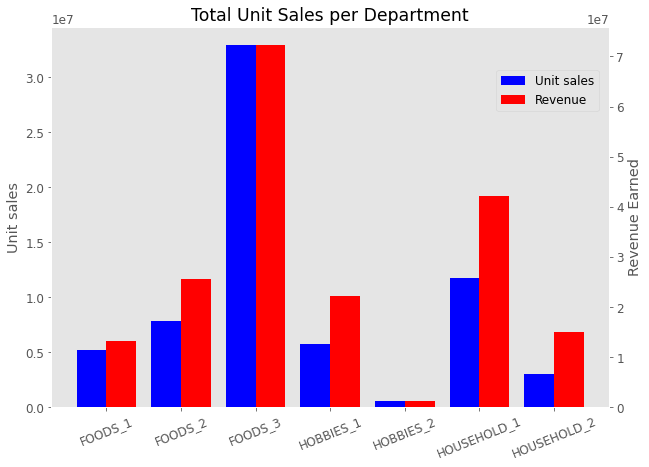
\includegraphics[width=0.52\textwidth]{figures/exploratory_data_analysis/sales_rev_depts.png}}
    \caption{Proportion of units sold and revenue earned per store.}
    \label{fig:depts_rev_stores}
    \vspace{-10pt}
\end{wrapfigure}
There are a total of seven departments in the dataset. 
There are three departments for the \texttt{FOODS} category, two departments for the \texttt{HOBBIES} category, and two departments for the \texttt{HOUSEHOLD} category.
The number of unit sales and revenue earned in each department is compared in Figure \ref{fig:sales_rev_depts}
The bar chart shows that .... .
Moreover, Figure \ref{fig:dept_sales} shows a 30-day moving average of the number of sales per department, which shows that the \textit{FOODS\_3} department has a higher number of unit sales, as well as a higher volatility compared to the other departments.

\begin{figure}[H]
    \centering
    \fbox{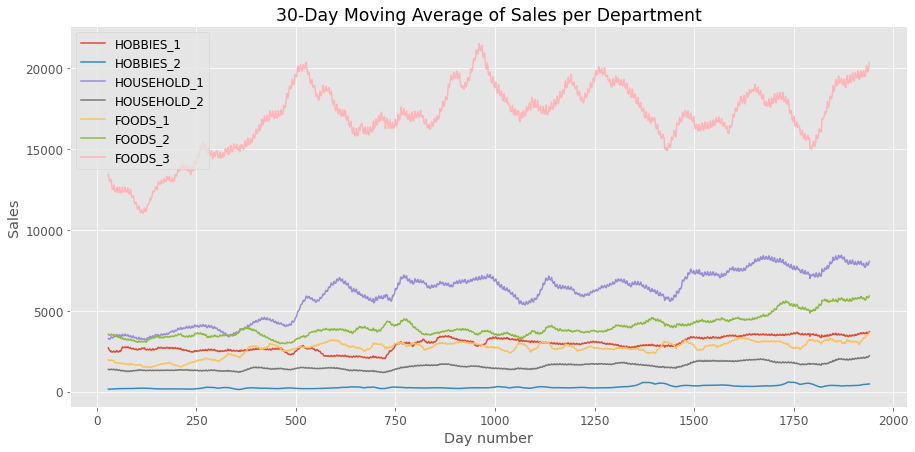
\includegraphics[width=0.98\textwidth]{figures/exploratory_data_analysis/dept_sales.png}}
    \caption{30-day moving average of sales per store.}
    \label{fig:dept_sales}
\end{figure}



\chapter{Methodology}
\section{Aim of Study}
The data contains a time-series of the number of sales for 3049 products across 10 different stores, for a total of 30490 items. 
We aim to create several models and compare their performance on predicting the number of sales for all 30490 items for the next 28 days. 
Specifically, we aim to compare the performance of deep learning and machine learning methods.
For deep learning methods, we will compare the performance of Recurrent Neural Networks (RNN) with Artificial Neural Networks (ANN). 
Specifically, the recurrent neural network will be a Long Short-Term Memory (LSTM) model, and the artificial neural network will be a Multi-Layer Perceptron (MLP) model.
Moreover, the machine learning method was chosen to be a LightGBM (LGBM) model. 
Additionally, we will create a hybrid model, consisting of the LSTM model and the best performing model between the MLP and LGBM models, and check if it is able to improve the performance compared to the sigular models.


\section{Selection of the Response Variable}
All models will be trained using the Root Mean Square Error (RMSE) as the loss function.
Moreover, the RMSE on the validation set will be used to optimize the hyperparameters of each model.
On the other hand, in order to evaluate and compare the performances of the models, we will obtain the Root Mean Square Scaled Error (RMSSE) of the models on the test set.
Compared to RMSE, RMSSE has the advantage of being scale independent, and so it can be used to compare the accuracy of forecasts across time-series with different scales.
For example, an absolute error of 10 when approximating 100 should have a much higher forecast error than an absolute error of 10 when approximating 1,000,000.
RMSSE is derived from the Mean Absolute Scaled Error (MASE), which is a common measure of accuracy for forecasting problems.
In order to scale the error, the Mean Squared Error (MSE) of the model is compared to the MSE of a naive model, which predicts the sales at each time-step to be the same as the previous time-step.
The original RMSSE uses the in-sample data (training set) for the naive model, since the out of sample data (test set) may not contain enough points to obtain a naive prediction when the forecasting horizon is too short: \cite{yardstick, m5}
\[RMSSE = \sqrt{\frac{MSE_{\,test, \,model}}{MSE_{\,train, \,naive}}}\]
However, since in our study we have a forecasting horizon of 28, we do not have to worry about this issue and hence for simplicity, we will use the out of sample data to obtain the MSE of the naive model:
\[RMSSE = \sqrt{\frac{MSE_{\,test, \,model}}{MSE_{\,test, \,naive}}}\]

Another advantage of RMSSE compared to RMSE is its interpretability. 
The value of RMSSE represents how well a model performs compared to a naive model. 
An \(RMSSE > 1\) means that the model performs worse than the naive model and should be discarded, an \(RMSSE = 1\) means the model performs just as well as the naive model, and an \(RMSSE < 1\) means the model performs better than the naive model. 
The closer the value of RMSSE is to 0, the better the model performs.

In addition to RMSSE, the Mean Error (ME) of the models will be obtained in order to see whether the models have a tendency to over-forecast or under-forecast the target sale values.

\section{Choice of Factors and Levels}
The following four models will be evaluated and compared in this project.

\begin{enumerate}
  \item LSTM,
  \item Artificial Neural Network,
  \item LightGBM, and
  \item Hybrid.
\end{enumerate}

The hyperparameters of all models will be optimized using Bayesian Optimization over a given range of hyperparameter values.
In Bayesian optimization, the optimizer starts with a prior belief of the environment and with every combination of hyperparameter values that it examines, it updates its belief of the environment and looks for the hyperparameter values that will maximize the chance of improving our performance in the next round. 
For the LSTM and MLP models, Bayesian optimization was used to optimize the number of hidden layers, number of hidden units, learning rate, learning rate decay, dropout rate, and batch size.
Moreover, Bayesian optimization was used to decide whether a batch normalization layer should be included in the architecture of the models. 
Additionally, the number of historical observations for the LSTM model was optimized as well.
On the other hand, the LGBM model has many hyperparameters that can be optimized. 
In this project, Bayesian optimization was used to find the best hyperparameter values for the learning rate, the fraction of the features used, the value of lambda for L2 regularization, the minimum data in each leaf, and the number of leaves for the model.

\section{Choice of Experimental Design}
The time-series include a total of 1941 days of sales data, which will be split into training, validation, and test sets. 
The training set will include 1885 days of time-series data, which will be used to train the hybrid model.
The validation set will include a time-series data for the next 28 days, from day 1886 to day 1913, which will be used for hyperparameter optimization.
Finally, the test set will include the last 28 days of time-series data, from day 1914 to day 1941, which will be used to evaluate and compare the models and assess their generalization on unseen data. 

Since the dataset contains the sales data for 3049 products sold across ten different stores, we are dealing with a multi-channel problem. 
It is important to take into account the effects of aggregate demand on the sales, as well as the effects of one items on the sales of another item.
Hence, rather than training separate models for each item, a single model will be created for all items.
Furthermore, since we want to forecast the daily sales for the next 28 days, we are dealing with a multi-step forecasting problem. 
There are three main methods for dealing with multi-step forecasting problems.
In the first method, a separate model is trained for each step. 
However, this is not very practical, not only because of the number of models that will need to be trained, but also because normally the sales on each day are somehow dependent on the sales of the previous days, which is not considered in this method.
In the second method, a single model predicts all steps at once.
However, this method also lacks the ability to obtain any information from the previous steps of the forecasting horizon to predict future steps.
Alternatively, one can use a single model to forecast each step one at a time, where at each step, the previous forecasted values are used to forecast the sales of the current day.
This method can be more consistent as it takes into account the effects of previous days when forecasting many days ahead.
Hence, this is the method that will be used in this project to deal with multi-step forecasting.

In the rest of this section, we will talk about the two experiments that will be performed in this project.

\subsection*{Experiment 1}
Three singular models (LSTM, MLP, and LGBM) will be constructed and their performances will be evaluated and compared for 28-days ahead point forecasts. 
In order to help the MLP and LGBM models learn the seasonality from the time-series data and look more than one step in the past, we will introduce lag features in the dataset. 
To produce lag features, we will shift the sales data to the future by a fixed number of days. 
For example, the lag 7 of the sales at time-step \(t\) for an item will be its sales value at time-step \(t-7\). 
In addition to the lag features, we will introduce rolling means and rolling standard deviations of the sales with various sliding-window sizes in order to help the models learn from the time-series data.

\subsection*{Experiment 2}
For the second experiment, a hybrid model will be constructed and its performance will be compared with the performances of its two components.
There are two elements in the dataset that must be considered when constructing the model's architecture.
The first element is the time-series data and the second element is all other data, such as promotions and holidays, that are considered to be external factors and might have an influence on the time-series data.
Hence, the first component of the hybrid model will be the LSTM network that will learn from the time-series data. 
LSTM networks are able to handle both the linear and nonlinear demand variations, which eliminates the need of multiple methods for different demand variations \cite{c8}.
The second component of the hybrid model will serve to learn from the external factors. 
Specifically, the second component will predict the difference in LSTM's predictions and actual demand based on the external factors.
To elaborate, assume we want to predict the demand for a time period, \(t \geq 1\), with the actual demand data, \(Y_t\), known. 
If the LSTM model makes predictions, \(\hat{y_t}\), for this time period, then the difference in the LSTM's predictions and the actual demand is calculated as:
\[\Delta y_t = Y_t - \hat{y_t}\]
This difference, \(\Delta y_t\) will be used as the independent variable(s) in the second component of the hybrid model, along with the external factors as the dependant variables. The second component will then be trained to predict this difference, \(\Delta \hat{y_t}\), based on the external factors. At last, the final forecast, \(\hat{Y_t}\), will be obtained by aggregating the predictions of the two model components \cite{c8}:
\[\hat{Y_t} = \hat{y_t} + \Delta \hat{y_t}\]
The study done in \cite{c8} has already used a Random Forest (RF) network as the second component for forecasting demands of a multi-channel retail, and they were able to achieve very accurate predictions.
In this study, we will use the best performing model between MLP and LGBM as the second component of the hybrid model. 
Similar to random forest, LGBM is a tree-based learning model, however, LGBM uses gradient boosting to enhance the performance of the model, whereas random forest uses bagging.

\section{Technologies}
All models will be created using \texttt{Python}. 
The LSTM and ANN models will be constructed using the package \texttt{keras} and LGBM will be implemented using the package \texttt{lightgbm}. 
The Bayesian optimization will be created using the \texttt{bayesian-optimization} package.
Moreover, other packages, such as \texttt{pandas} and \texttt{scikit-learn}, will be used for data preprocessing and model evaluation.


\chapter{Results}
The following four models were constructed: 
\begin{enumerate}
    \item Long Short-Term Memory (LSTM)
    \item Multi-Layer Perceptron (MLP)
    \item LightGBM (LGBM)
    \item LSTM-LGBM Hybrid
\end{enumerate}
Bayesian optimization was used to optimize the hyperparameters of the models within a given range of values.
The optimization process consisted of a few rounds of exploration, where new points are randomly explored within the available space, and many rounds of exploitation, where Bayesian optimization is done to find the optimal hyperparameters.
The performances of the optimized models were evaluated on the training, validation and test sets for a 1-day ahead point forecast and were compared to the performance of a naive model.
Moreover, the performance of each optimized model was evaluated on the test set for a 28-days ahead point forecast and compared to the naive model.
The ME, RMSE, and RMSSE of each model after hyperparameter optimization on the training, validation, and test sets are shown in tables \ref{tab:lstm_results}, \ref{tab:ann_results}, \ref{tab:lgbm_results}, \ref{tab:hyb_results}.
Note that for the MLP and LGBM models, the 1-day ahead forecasts are the same as the 28-days ahead forecasts, but for the LSTM and hybrid models, these forecasts are different.
This is due to the difference in the feature engineering done for the LSTM and hybrid models compared to the MLP and LGBM models, which will be discussed further in the discussion.
% talk more about which model fitted best on the trn/val/tst sets. whether it was able to generalize as well?
From the results, it can be seen that the LGBM model outperforms the other models with an RMSSE of \lgbmTstMonRMSSE{} on the test set for 28-days ahead forecasts.

In the rest of this chapter, the results of hyperparameter optimization and the performance of each model on the training, validation, and test sets will be discussed in detail. 

\section{Long Short-Term Memory}
\InsertBoxR{3}{
    \parbox{0.5\linewidth}{
    \vspace{4mm}
    \captionsetup{width=0.49\textwidth}
    \fbox{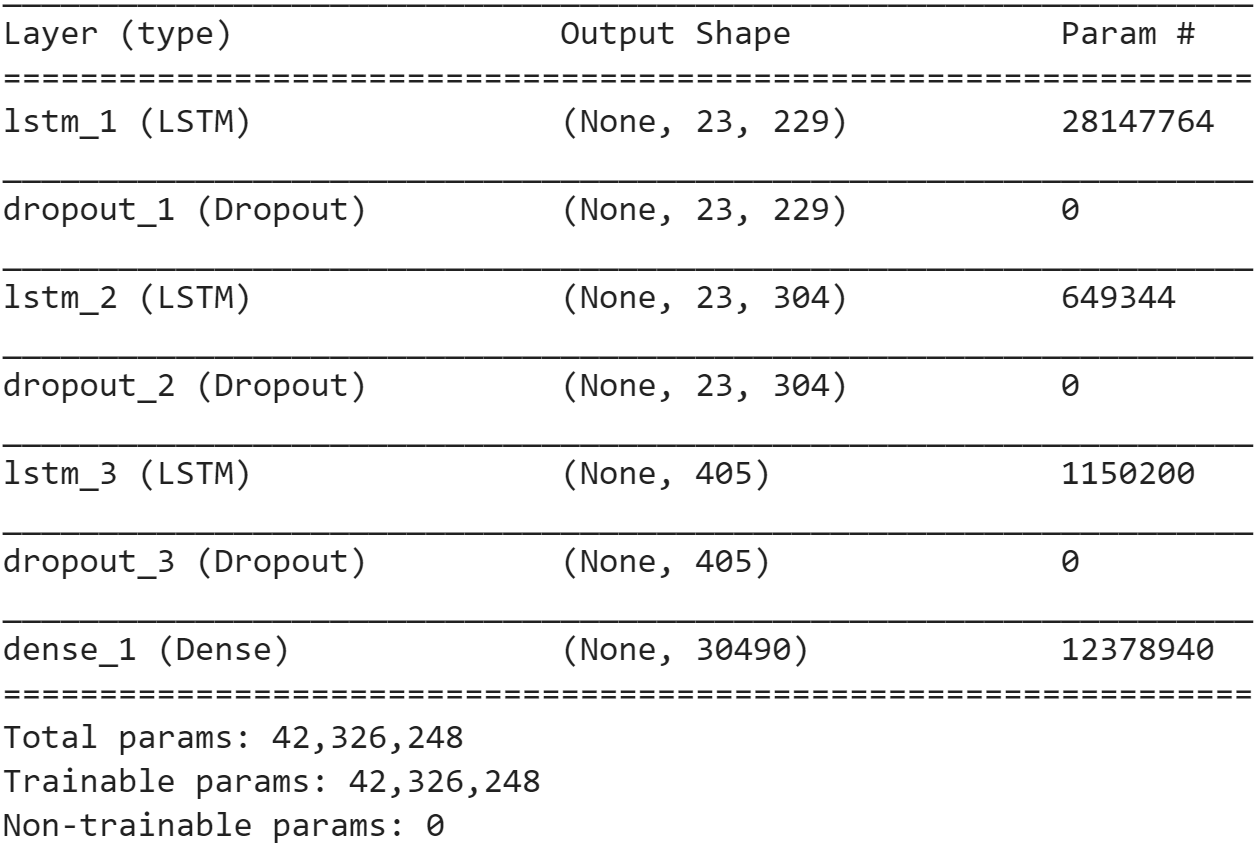
\includegraphics[width=0.47\textwidth]{figures/results/lstm_summary.PNG}}
    \captionof{figure}{A summary of the LSTM's structure.}
    \label{fig:lstm_summary}}}[3]
Figure \ref{fig:lstm_summary} shows a summary the LSTM model's structure. 
The LSTM model was able to achieve an RMSE of \lstmTrnRMSE{} on the training set, \lstmValRMSE{} on the validation set, and \lstmTstRMSE{} on the test set, when predicting one day ahead. 
Moreover, the RMSE of the model on the test set for 28-days ahead forecasts was \lstmTstMonRMSE{}.
Figure \ref{subfig:lstm_sample1} shows the 1-day ahead predictions of the LSTM model versus the actual sale values for the last 28 days of the training set, as well as the entire validation and test sets, which shows that the model was able to learn the weekly pattern presented in the time-series data.
The 28-days ahead predictions of the model on the test set are also shown in Figure \ref{subfig:lstm_sample28}.
From these predictions, we can see that the model struggles to forecast the last days of the horizon and starts to lose its weekly pattern.
This is most likely due to error propagation from the earlier predictions, which will be discussed further in the discussion.

Figure \ref{fig:lstm_curve} shows the learning curve of the model on the training and validation sets. 
It can be seen that the RMSE of the model plateaus around epoch 20, and the best validation RMSE occurs at epoch 23.
Moreover, the RMSSE of the 28-days ahead forecasts on the test set was \lstmTstMonRMSSE{}, which means that the model was able to perform around 20.5\% better than the naive model, and the ME of 28-days ahead forecasts on the test set was \lstmTstMonME{}, which means that the model has a tendency to under-forecast the target sale values. 

Using Bayesian optimization, the number of historical observations was optimized to be \lstmParamsSteps{} days, and a batch size of \lstmParamsBatch{} was chosen for the training process. 
Moreover, the optimized LSTM structure contained three hidden LSTM layers with 229, 304, 405 nodes, respectively. 
The dropout rate was optimized to be \lstmParamsDropout{}, however, no batch normalization layers were included.
Finally, the learning rate was optimized to be \lstmParamsLR{} with a decay rate of \lstmParamsDecay{}. 
Table \ref{tab:lstm_params} shows the range of values that each hyperparameter was optimized over, as well as the optimized values.


\section{Multilayer Perceptron}
% \begin{wrapfigure}{r}{0.5\textwidth}
%     \vspace{-5pt}
%     \centering
%     \captionsetup{width=0.47\textwidth}
%     \fbox{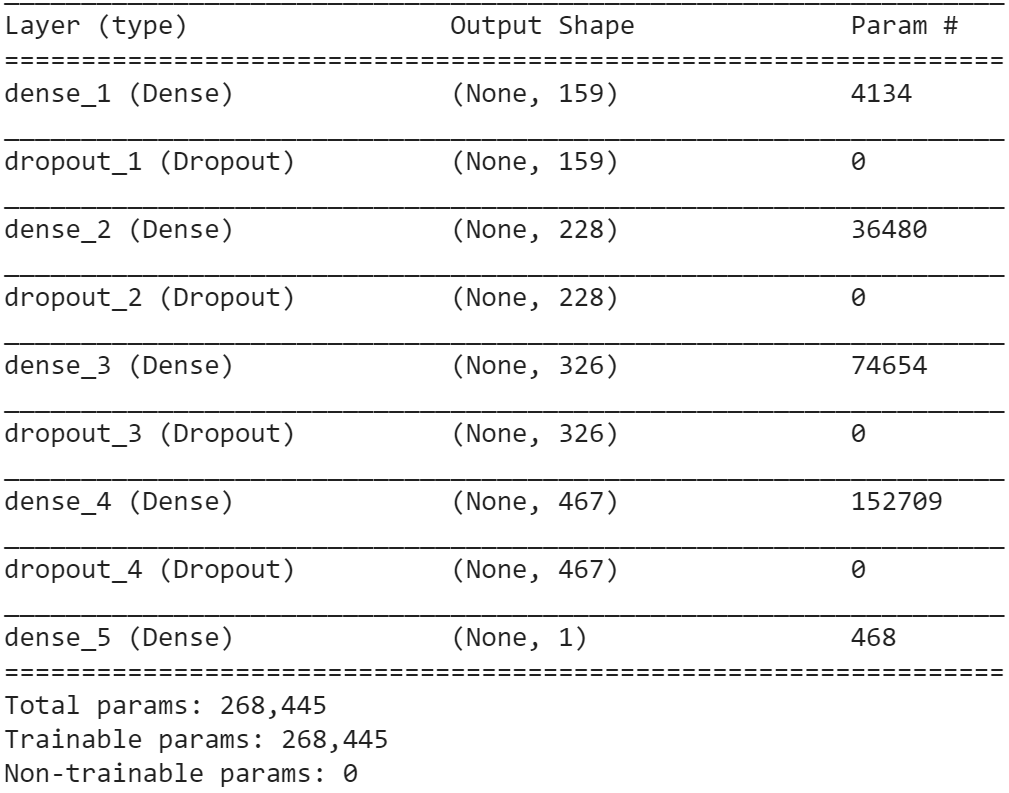
\includegraphics[width=0.47\textwidth]{figures/results/ann_summary.PNG}}
%     \caption{A summary of the MLP's structure.}
%     \label{fig:ann_summary}
%     \vspace{-10pt}
% \end{wrapfigure}
\InsertBoxR{3}{
    \parbox{0.5\linewidth}{
    \vspace{2mm}
    \fbox{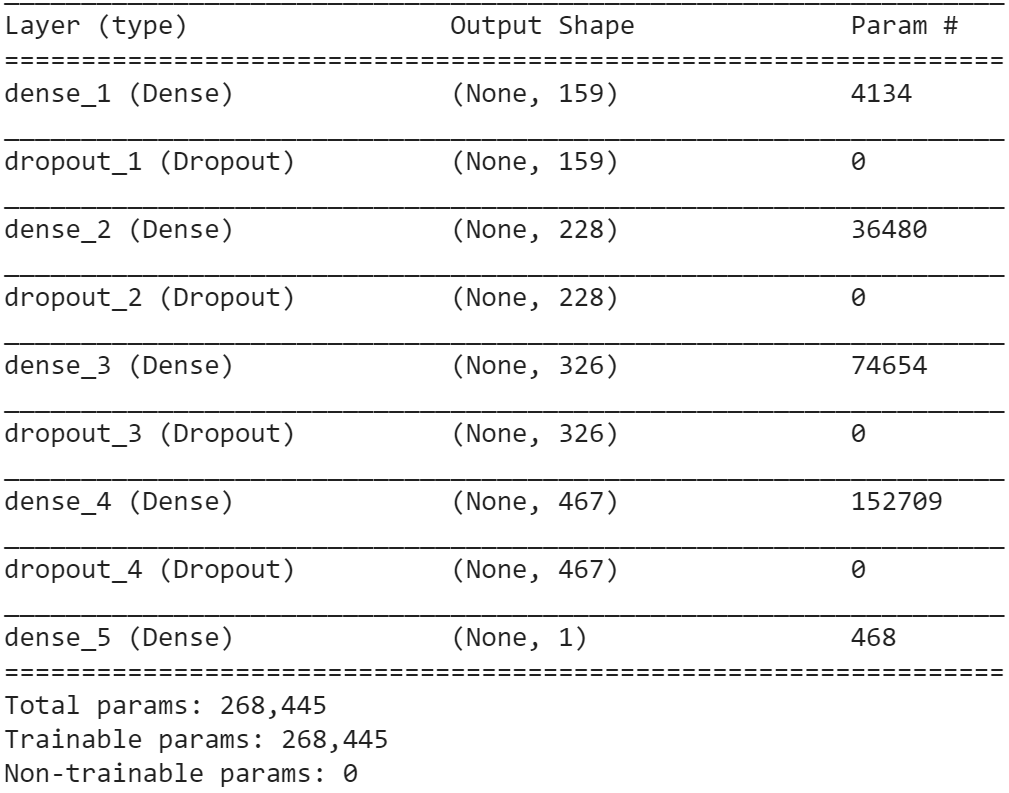
\includegraphics[width=0.47\textwidth]{figures/results/ann_summary.PNG}}
    \captionof{figure}{A summary of the MLP's structure.}
    \label{fig:ann_summary}}}[3]
A summary of the MLP model's structure is shown in Figure \ref{fig:ann_summary}.
The RMSE of the MLP model on the training, validation, and test sets were \annTrnRMSE{}, \annValRMSE{}, and \annTstRMSE{}, respectively.
Figure \ref{fig:ann_curve} shows the RMSE of the MLP model at each epoch on the training and validation sets.
This learning curve shows that most of the learning was done on the first iteration, and that the model had a difficult time learning useful information that will generalize well on the validation set after the first iteration.
The RMSE of the model exhibits a lot of oscillations, with the minimum validation error occurring at epoch 52.
Moreover, the MLP model was able to achieve an RMSSE of \annTstMonRMSSE{} for the 28-days ahead forecasts and was able to perform around 18.9\% better than the naive model.
Furthermore, the ME of the model on the test set was \annTstME{}, which means that the model has a tendency to under-forecast the target sale values.

The range of values that each hyperparameter of the model was optimized over, as well as their optimized values are shown in Table \ref{tab:ann_params}. 
The optimized MLP model contained four hidden fully-connected layers with 159, 228, 326, and 467 nodes, respectively.
Moreover, the optimized model did not include any batch normalization layers but had a dropout layer with a rate of \annParamsDropout{} after each fully-connected layer.
Additionally, for the training phase, the learning rate was optimized to be \annParamsLR{} with a decay rate of \annParamsDecay{} and the training batch size was optimized to be \annParamsBatch{}.


\section{LightGBM}
The LGBM model was able to achieve an RMSE of \lgbmTrnRMSE{}, \lgbmValRMSE{}, and \lgbmTstRMSE{} on the training, validation, and test sets, respectively.
The LGBM model was able to achieve the best performance on the test set compared to the other models.
From the learning curve of the model, shown in Figure \ref{fig:lgbm_curve}, it can be seen that the model's error plateaus around epoch 30, however, the model still continues to learn at a very low rate until epoch 122, where it reaches its best validation error, and then starts to overfit on the training set.
In addition, the ME and RMSSE of the 28-days ahead forecasts on the test set were \lgbmTstMonME{} and \lgbmTstMonRMSSE{}. respectively.
The RMSSE of the model shows that it was able to perform around 22.7\% better than the naive model.
Furthermore, the ME of the model shows that the model has a tendency to under-forecast the target sale values.

Table \ref{tab:lgbm_params} shows the range of values that each hyperparameter was optimized over and their optimized values.
The final LGBM model had a learning rate of \lgbmParamsLR{}, with \lgbmParamsFeatFrac{} fraction of features used to train each tree, and a lambda value of \lgbmParamsLambda{} for L2 regularization.
Moreover, the number of leaves for the model was chosen to be \lgbmParamsNleaves{} with a minimum data of \lgbmParamsMinData{} in each leaf.


\section{LSTM-LGBM Hybrid}
An LSTM model was chosen as the first component of the hybrid model in order to learn from the sales time-series data. 
Moreover, the best performing singular model between MLP and LGBM was used as the second component of the hybrid model.
Additionally, the optimal hyperparameters found previously for each singular model were used as the hyperparameters for each component.
The proposed hybrid model was able to obtain an RMSE of \hybTrnRMSE{} on the training set, \hybValRMSE{} on the validation set, and \hybTstRMSE{} on the test set for the 1-day ahead point forecasts.
These performances correspond to an RMSSE of \hybTrnRMSSE{}, \hybValRMSSE{}, and \hybTstRMSSE{} on the training, validation, and test sets, respectively.
Moreover, the RMSE and RMSSE of the hybrid model for the 28-days ahead forecasts on the test set were \hybTstMonRMSE{} and \hybTstMonRMSSE{}, respectively, which shows that the model was able to perform around 20.3\% better than the naive model.
Even though the hybrid model performed slightly worse than the singular LSTM model on the 1-day ahead forecasts, the hybrid model was able to obtain a slightly better performance on the 28-days ahead predictions, which shows that the second component, LGBM, was able to help counteract the effects of error propagation, which can be confirmed by comparing Figures \ref{subfig:lstm_sample28} and \ref{subfig:hyb_sample28}. 
On the other hand, the hybrid model was not able to beat the performance of the singular LGBM model.
Moreover, the ME of the model for the 28-days ahead forecasts on the test set was negative with a value of \hybTstMonME{}, which shows that the model is slightly under-forecasting the targets sale values.


\chapter{Discussion}
The hyperparameters of the models were optimized using Bayesian optimization.
Due to the very large dataset and the time constraint, all models were run for 100 iterations with an early stopping rounds of 10 during the optimization phase. 
However, during the training phase, all models were run for 1000 iterations with an early stopping rounds of 20, in order to maximize the learning done by the models.
On another note, for the LSTM and MLP models, optimizing the number of layers and the number of nodes per layer at the same time using Bayesian optimization is not a straightforward task.
In order to optimize these hyperparameters, Bayesian optimization was given a specific model structure, in which the number of nodes decrease by a certain factor when going from the last hidden layer to the first.
The Bayesian optimization was then used to optimize the number of layers, the number of nodes for the last hidden layer, as well as the decay rate of the number of nodes.
As a result, Baysian optimization did not have full flexibility over the model's structure. 
For example, a model with three layers and 64, 128, 128 nodes per layer cannot be created using the model structure described, and hence, it is possible that another model exists with a better performance that does not follow the specified model structure.
Moreover, different model structures have different learning patterns depending on their complexity. 
Simple models are able to learn quickly but plateau at a higher error value, whereas complex models learn slowly but can plateau at a lower error value.
Since the models were only ran for 100 iterations and 10 early stopping rounds during the optimization phase, it is possible that a better but more complex model did not have enough time to plateau.
Therefore, a better model can possibly be found by giving more flexibility over the structure of the model, exploring a higher range of values for each hyperparameter, as well as increasing the number of iterations and early stopping rounds during the optimization phase.

Furthermore, looking at Figures \ref{fig:lstm_worst}, \ref{fig:ann_worst}, \ref{fig:lgbm_worst}, and \ref{fig:hyb_worst}, we can see that the models have a difficult time forecasting the sales for the \texttt{FOODS\_3} department.
This shows that items in the \texttt{FOODS\_3} department do not follow the same patterns as the other items.
This can be confirmed by examining Figure \ref{fig:dept_sales}, which shows the difference in the patterns of sales between the \texttt{FOODS\_3} department and the other departments.
Not only do the items in the \texttt{FOODS\_3} department have higher sales, but they also show a seasonality pattern that is less visible in the other departments.
Hence, a possible way to improve forecasting accuracies is to train a separate model for items belonging to the \texttt{FOODS\_3} department.

LSTM models have a high reputation in learning from time-series data. 
However, the LSTM model did not perform as well as expected in this project.
This can be due to the fact that recurrent neural networks, such as LSTM, require extensive non-sparse data.
However, in our case, the data contains many zeros, which can significantly hinder the performance of the LSTM model.
Moreover, the LSTM model was very sensitive to the values of its hyperparameters, and hence, it requires extensive hyperparameter optimization.
On the other hand, LightGBM models are easy to train and are able to achieve a relatively good performance without much hyperparameter optimization.
Although the results of the LGBM model are noteworthy and show the strength of boosting methods in improving the overall performance, it is possible that a well optimized LSTM model can outperform the LGBM model, however, this would require a considerable amount of hyperparameter optimization.

Similarly, the hybrid model was not able to meet expectations. 
The performance of the hybrid model seemed to be very closely tied to the performance of its first component, LSTM, which is possibly due to the fact that the first component receives the main sales data and hence carries out the main learning in the model.
Moreover, although the second component, LGBM, was able to slightly improve the accuracy of the 28-days ahead forecasts, it was not able to learn much from the residual data that was provided and seemed to have a difficult time finding a pattern and predicting the error of the LSTM model.
Therefore, it could be possible for the hybrid model to beat the performance of its two individual components, however, its first component will need to perform at least as good as its second component when used as a singular model, since the first component will be doing the main learning in the hybrid model.
Furthermore, another possible way to improve the performance of the hybrid model is to perform hyperparameter optimization on its two components.
In this project, the hyperparameters of the singular models were used in the hybrid model.
Since the input data for the two components are similar to the input data of the singular models, this can be considered a case of transfer learning, and hence the same hyperparameters should be able to perform relatively well.
However, with further hyperparameter optimization, we should still be able to find better hyperparameters for each component of the hybrid model.
Nevertheless, hybrid models are not guaranteed to outperform singular models and model selection has a significant influence on their performance as well \cite{c12}.

Another factor to consider when evaluating the performances is the choice of features used.
The main data for the LSTM model included the sales time-series for each item, which is what the model will be predicting. 
In order to help with the predictions for the singular LSTM model, seven other features were used from the dataset, and two additional features were introduced. 
The seven features used from the dataset include the current day number, weekday, month, year, SNAP days for California, SNAP days for Texas, and SNAP days for Wisconsin. 
Moreover, two additional features were created from the available events data, which represented whether an event exists on the day of the prediction, and whether an event exists the day after the prediction.
The reason that the model was provided with information about the events of the next day is that people tend to go shopping before an event rather than the day of the event.
For example, in case of Halloween, a lot of people tend to buy their candies before Halloween starts rather than on the day of Halloween.
Moreover, we also tried providing the model with the price information of each item, as well as the exact name and type of each event, however, the performance of the LSTM model was significantly hindered, and hence, these features were omitted.
This is possible due to the large number of features added, since there is a new feature added for the price of each item, and hence, we are essentially doubling our feature set.

\begin{figure}[b!]
    \centering
    \fbox{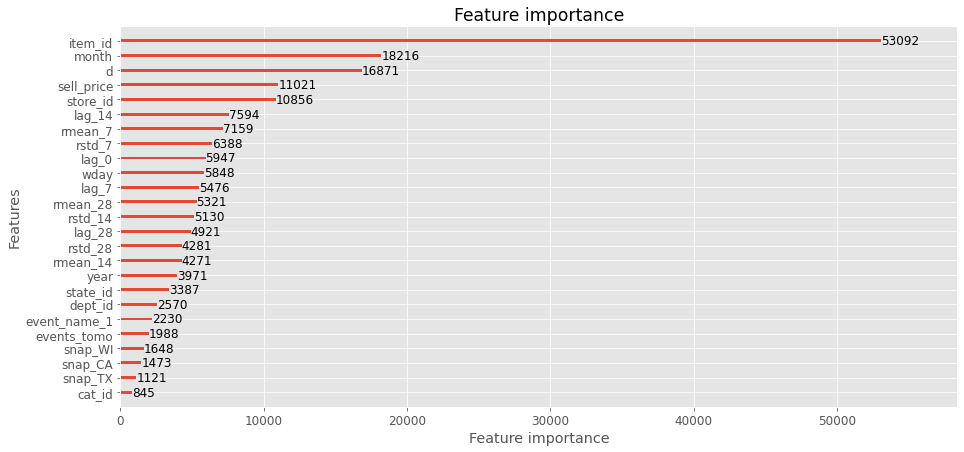
\includegraphics[width=0.95\textwidth]{figures/results/feat_importance.png}}
    \caption{The importance of each feature obtained from the LGBM model.}
    \label{fig:feat_imp}
\end{figure}
For the MLP and LGBM models, all available features were used. In addition, the lag of sale values with intervals 28, 35, 42, and 56 days, and the rolling mean and standard deviation of the sale values with window sizes 7, 14, and 28 days and a lag of 28 days were introduced.
Figure \ref{fig:feat_imp}, which was obtained from the singular LGBM model, shows a list of these features and their significance in attaining the predictions.
Note that all lag and rolling mean/std features were shifted by 28 days, since we have a forecasting horizon of 28 days.
Shifting these features by the value of the forecasting horizon prevents the error of the model to propagate through later predictions.
For example, if we introduce a lag feature with an interval of 7 and try to predict 28 days ahead, we will not have the actual sale values after the seventh forecast and we will have to use the predicted values instead. 
This means that if there is an error in the predictions, the error will propagate through later forecasts as well.
However, we also tried providing the MLP and LGBM models with lag and rolling mean/std features that are within the forecasting horizon. 
Even though this boosted the performances on the 1-day ahead forecasts, it significantly hindered the performances on the 28-days ahead forecasts.
Although, it is important to note the importance of recent sales in the foretelling the future sales. 
Having knowledge of recent sale values can greatly help with the predictions, however, this comes with the trade-off of error propagation when forecasting longer horizons.
Therefore, further optimization can be possibly done by providing the models with lag and rolling mean/std features that are within the forecasting horizon and balancing the aforementioned trade-off between the recency of these features and error propagation.
Moreover, the reason that the 1-day and 28-days ahead forecasts of the MLP and LGBM models are the same is the fact that all lag and rolling mean/std features are shifted by the value of the forecasting horizon, and so actual sale values are available for the entire forecasting horizon.
However, this is not the case for the LSTM model, since the LSTM model will have to depend on its own predictions when it has a large forecasting horizon, and hence the LSTM and hybrid models obtain different 1-day and 28-days ahead predictions.


\chapter{Conclusions and Future Work}
The performance of the LGBM model highlights the potential of boosting methods in improving the overall performance. 
Compared to the MLP model, which had the same preprocessing procedure as the LGBM model, not only was the LGBM model easier to construct, but it was also able to train much faster, which shows the ability of LGBM models in working with large datasets.
Moreover, from the results of the LSTM and MLP models, we can clearly see the ability of LSTM models in working with time-series data compared to regular deep learning models.

Another goal of this paper was to evaluate the capabilities of hybrid models.
Unlike the study done in \cite{c8}, we did not find hybrid models to be useful for improving the performance.
In our case, the performance of the hybrid model was closely tied to the performance of its first component.
Future studies should further explore the capabilities of hybrid models and how much their performance depends on the performance of the first component.
Moreover, future work on this dataset can focus on further hyperparameter optimization and feature engineering to improve the performance of the LSTM model.

All models in this paper were trained on the entire dataset.
However, the results show that the models were unable to confidently forecast the sales for the \texttt{FOODS\_3} department. 
Hence, future studies studies can try to enhance the performances by training a separate model for the \texttt{FOODS\_3} department, or even one model per department.
It is however important to balance the number of models in order to not lose too much inter-dependency between the different item groups.


\end{ryerson}


\begin{appendices}

\chapter{Tables}

\begin{table}[h!]
    \centering
    \caption{LSTM hyperparameters ranges and their optimal values.}
    \resizebox{\textwidth}{!}{
    \begin{tabular}{ || c | c | c | c || }
        \hline
        Hyperparameter & Range & Optimal value & Description \Tstrut\Bstrut \\
        \hline
        n\_layers & \lstmParamsRangeNlayers & \lstmParamsNlayers & number of layers \Tstrut\\[0.5ex]
        last\_units  & \lstmParamsRangeNunits & \lstmParamsNunits & number of nodes for the last hidden layer \\[0.5ex]
        units\_decay & \lstmParamsRangeScale & \lstmParamsScale & decay rate of the number of nodes \\[0.5ex]
        learning\_rate & \lstmParamsRangeLR & \lstmParamsLR & learning rate of the model \\[0.5ex]
        lr\_decay & \lstmParamsRangeDecay & \lstmParamsDecay & decay rate of the learning rate \\[0.5ex]
        dropout\_rate & \lstmParamsRangeDropout & \lstmParamsDropout & dropout rate for the dropout layers \\[0.5ex]
        norm & \lstmParamsRangeNorm & \lstmParamsNorm & whether to add batch normalization layers \\[0.5ex]
        batch\_size & \lstmParamsRangeBatch & \lstmParamsBatch & batch size for the training phase \\[0.5ex]
        steps & \lstmParamsRangeSteps & \lstmParamsSteps & number of time steps for LSTM data \\[0.5ex]
        \hline
    \end{tabular}}
    \label{tab:lstm_params}
\end{table}

\begin{table}[h!]
    \centering
    \caption{MLP hyperparameters ranges and their optimal values.}
    \resizebox{\textwidth}{!}{
    \begin{tabular}{ || c | c | c | c || }
        \hline
        Hyperparameter & Range & Optimal value & Description \Tstrut\Bstrut \\
        \hline
        n\_layers & \annParamsRangeNlayers & \annParamsNlayers & number of layers \Tstrut\\[0.5ex]
        last\_units  & \annParamsRangeNunits & \annParamsNunits & number of nodes for the last hidden layer \\[0.5ex]
        units\_decay & \annParamsRangeScale & \annParamsScale & decay rate of the number of nodes \\[0.5ex]
        learning\_rate & \annParamsRangeLR & \annParamsLR & learning rate of the model \\[0.5ex]
        lr\_decay & \annParamsRangeDecay & \annParamsDecay & decay rate of the learning rate \\[0.5ex]
        dropout\_rate & \annParamsRangeDropout & \annParamsDropout & dropout rate for the dropout layers \\[0.5ex]
        norm & \annParamsRangeNorm & \annParamsNorm & whether to add batch normalization layers \\[0.5ex]
        batch\_size & \annParamsRangeBatch & \annParamsBatch & batch size for the training phase \\[0.5ex]
        \hline
    \end{tabular}}
    \label{tab:ann_params}
\end{table}

\begin{table}[h!]
    \centering
    \caption{LGBM hyperparameters ranges and their optimal values.}
    \resizebox{\textwidth}{!}{
    \begin{tabular}{ || c | c | c | c || }
        \hline
        Hyperparameter & Range & Optimal value & Description \Tstrut\Bstrut \\
        \hline
        learning\_rate & \lgbmParamsRangeLR & \lgbmParamsLR & learning rate of the model \Tstrut\\[0.5ex]
        feature\_fraction & \lgbmParamsRangeFeatFrac & \lgbmParamsFeatFrac & fraction of features used to train each tree \\[0.5ex]
        lambda\_l2 & \lgbmParamsRangeLambda & \lgbmParamsLambda & value of lambda for L2 regularization \\[0.5ex]
        num\_leaves & \lgbmParamsRangeNleaves & \lgbmParamsNleaves & maximum number of leaves in one tree \\[0.5ex]
        min\_data\_in\_leaf & \lgbmParamsRangeMinData & \lgbmParamsMinData & Minimum number of data in each leaf \\[0.5ex]
        \hline
    \end{tabular}}
    \label{tab:lgbm_params}
\end{table}
\chapter{Figures}

% ==========================================================================================
% Exploratory Data Analysis
% ==========================================================================================
\begin{figure}[H]
    \centering
    \fbox{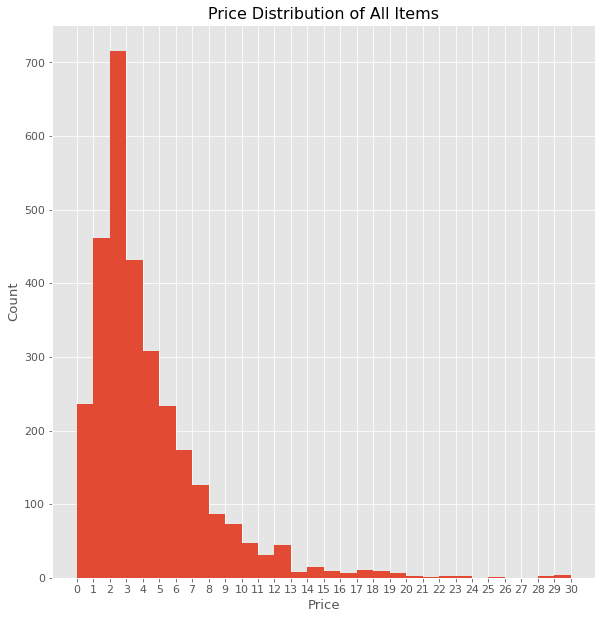
\includegraphics[width=0.9\textwidth]{figures/exploratory_data_analysis/price_all.png}}
    \caption{The distribution of the prices of all products.}
    \label{fig:price_all}
\end{figure}

\begin{figure}
    \centering
    \fbox{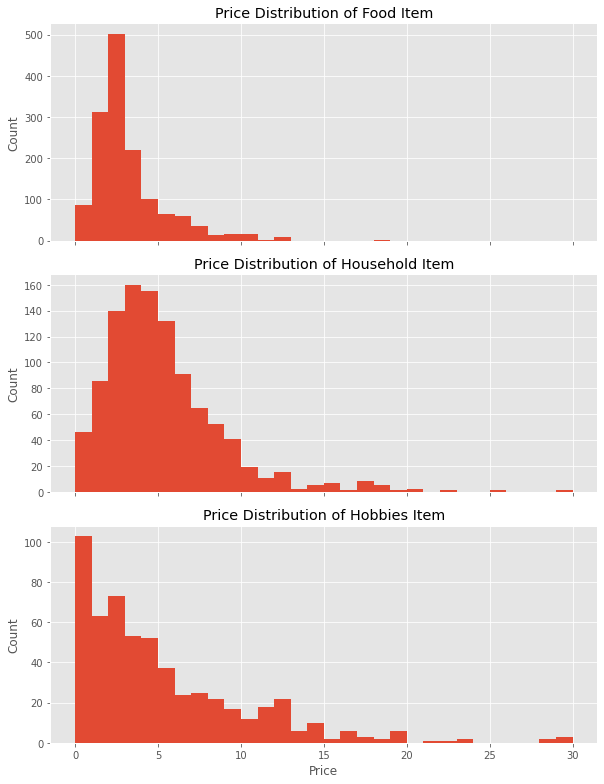
\includegraphics[width=0.98\textwidth]{figures/exploratory_data_analysis/price_dist_cats.png}}
    \caption{The price distribution of products in each product category.}
    \label{fig:price_cats}
\end{figure}

\begin{figure}
    \centering
    \fbox{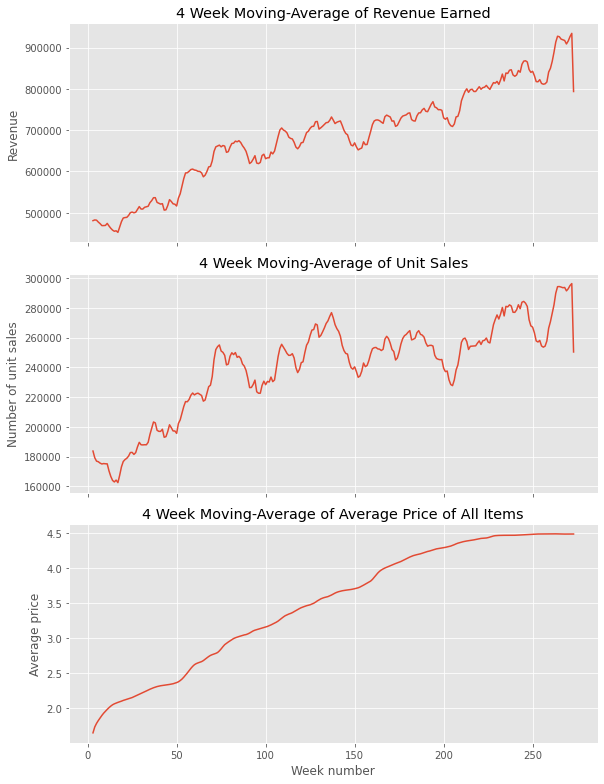
\includegraphics[width=0.98\textwidth]{figures/exploratory_data_analysis/4-week-ma.png}}
    \caption{4 week moving-average of revenue, unit sales, and average price of items.}
    \label{fig:ma_4week}
\end{figure}

% ==========================================================================================
% RESULTS
% ==========================================================================================

\begin{figure}
    \centering
    \fbox{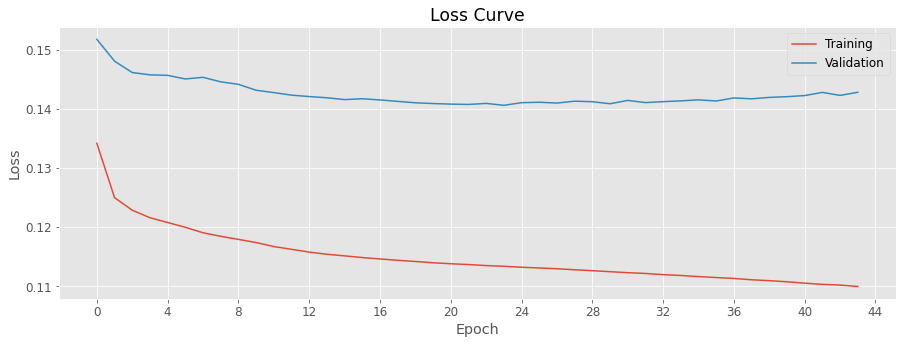
\includegraphics[width=0.95\textwidth]{figures/results/lstm_curve.png}}
    \caption{The learning curve of the LSTM model.}
    \label{fig:lstm_curve}
\end{figure}

\begin{figure}
    \centering
    \fbox{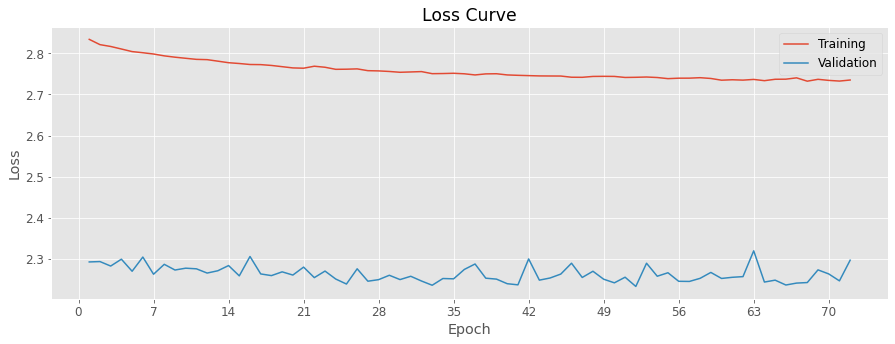
\includegraphics[width=0.95\textwidth]{figures/results/ann_curve.png}}
    \caption{The learning curve of the MLP model.}
    \label{fig:ann_curve}
\end{figure}

\begin{figure}
    \centering
    \fbox{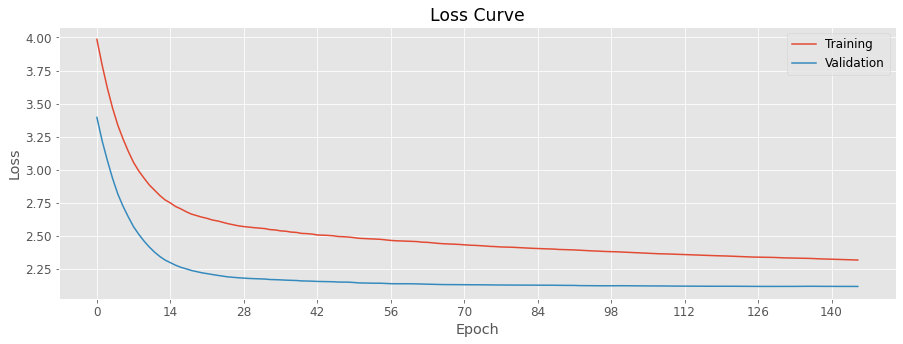
\includegraphics[width=0.95\textwidth]{figures/results/lgbm_curve.png}}
    \caption{The learning curve of the LGBM model.}
    \label{fig:lgbm_curve}
\end{figure}

\clearpage
\begin{figure}
\centering
    \subfloat[1-day ahead predictions on the training, validation, and test sets.]{
    	\label{subfig:lstm_sample1}
    	\fbox{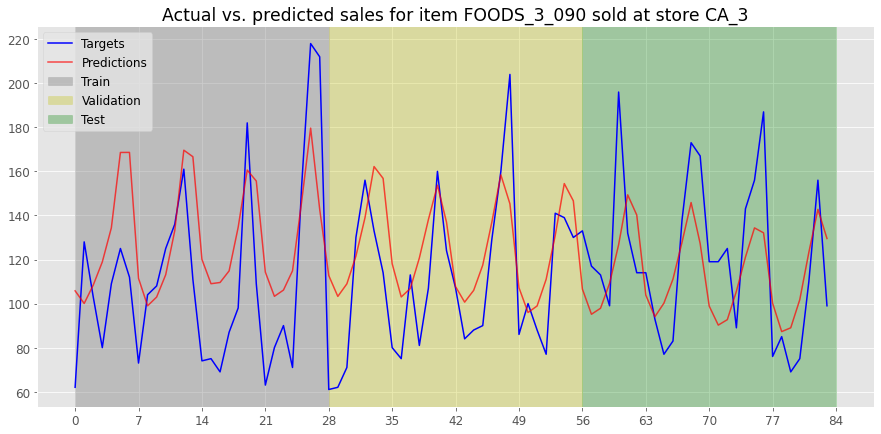
\includegraphics[width=0.95\textwidth]{figures/results/lstm_sample_preds.png}}
    	} 
    \vspace{5mm}
    \subfloat[28-days ahead predictions on the test set]{
    	\label{subfig:lstm_sample28}
    	\fbox{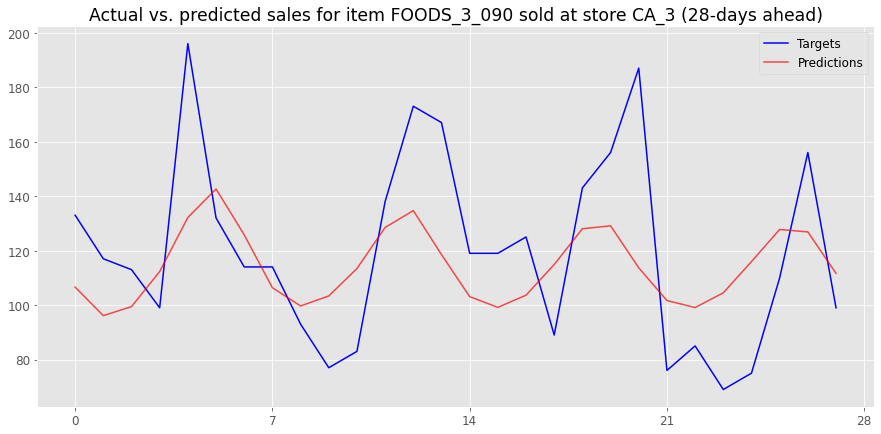
\includegraphics[width=0.95\textwidth]{figures/results/lstm_tst28_preds.png}}
    	}
    \vspace{2mm}
    \caption{Samples of LSTM predictions vs. the actual values.}
    \label{fig:lstm_samples}
\end{figure}

\begin{figure}
    \centering
    \fbox{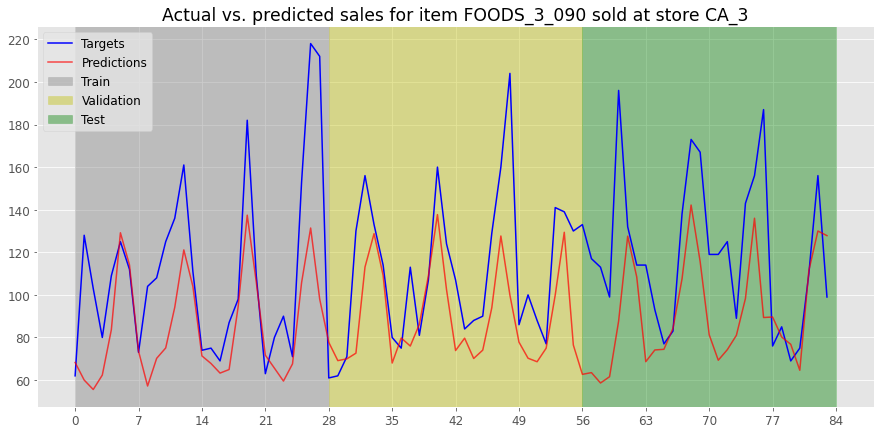
\includegraphics[width=0.95\textwidth]{figures/results/ann_sample_preds.png}}
    \caption{Samples of MLP predictions vs. the actual values.}
    \label{fig:ann_samples}
\end{figure}

\begin{figure}
    \centering
    \fbox{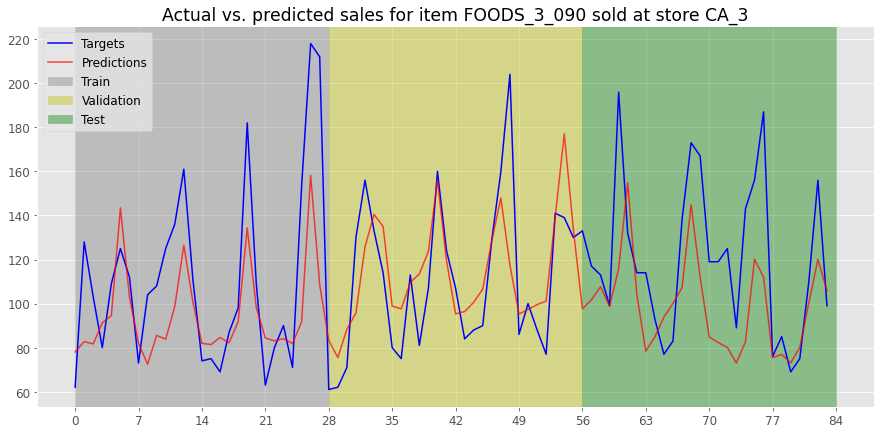
\includegraphics[width=0.95\textwidth]{figures/results/lgbm_sample_preds.png}}
    \caption{Samples of LGBM predictions vs. the actual values.}
    \label{fig:lgbm_samples}
\end{figure}

\begin{figure}
\centering
    \subfloat[1-day ahead predictions on the training, validation, and test sets.]{
    	\label{subfig:hyb_sample1}
    	\fbox{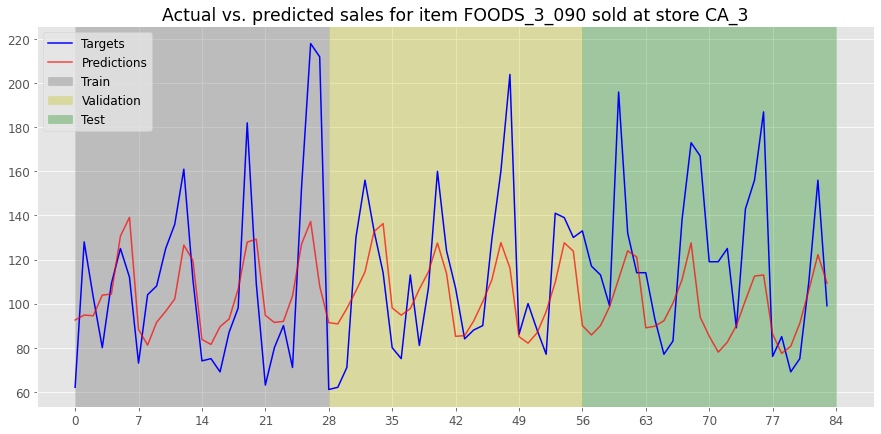
\includegraphics[width=0.95\textwidth]{figures/results/hyb_sample_preds.png}}
    	} 
    \vspace{5mm}
    \subfloat[28-days ahead predictions on the test set]{
    	\label{subfig:hyb_sample28}
    	\fbox{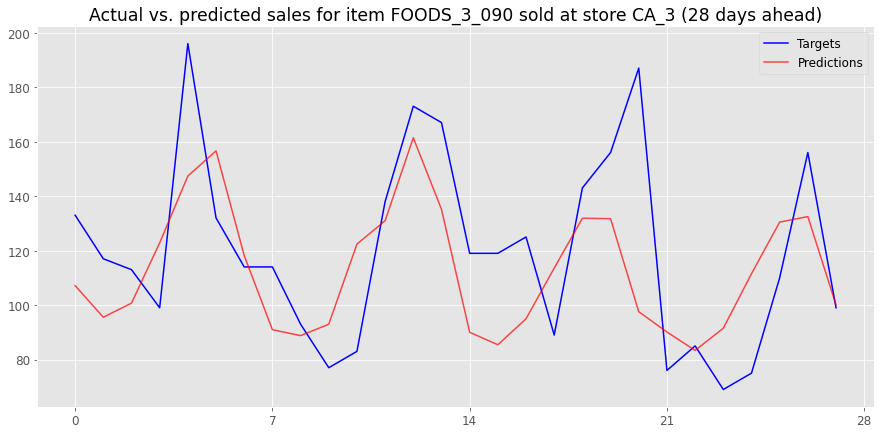
\includegraphics[width=0.95\textwidth]{figures/results/hyb_tst28_preds.png}}
    	} 
    \vspace{2mm}
    \caption{Samples of the LSTM-LGBM hybrid model's predictions vs. the actual values.}
    \label{fig:hyb_samples}
\end{figure}

\clearpage
\begin{figure}
    \centering
    \fbox{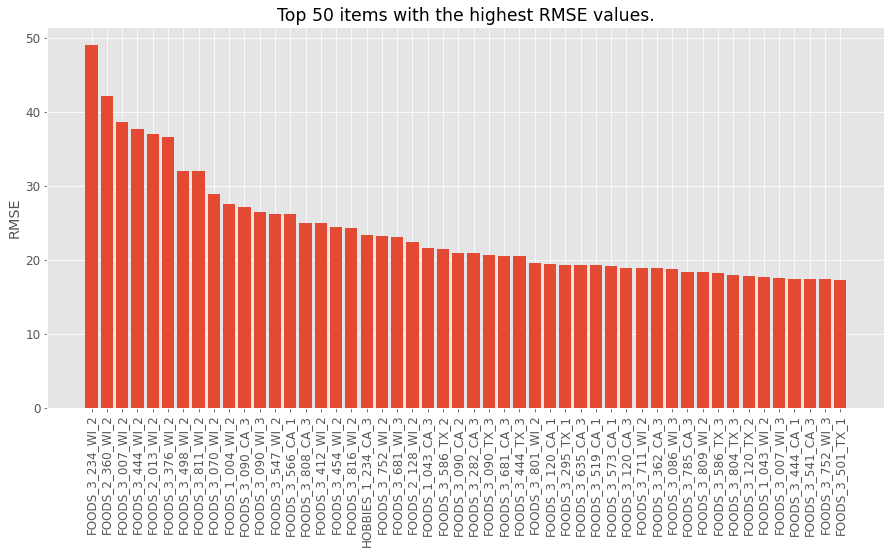
\includegraphics[width=0.95\textwidth]{figures/results/lstm_worst.png}}
    \caption{Top 50 items with the highest RMSE for the LSTM model.}
    \label{fig:lstm_worst}
\end{figure}

\begin{figure}
    \centering
    \fbox{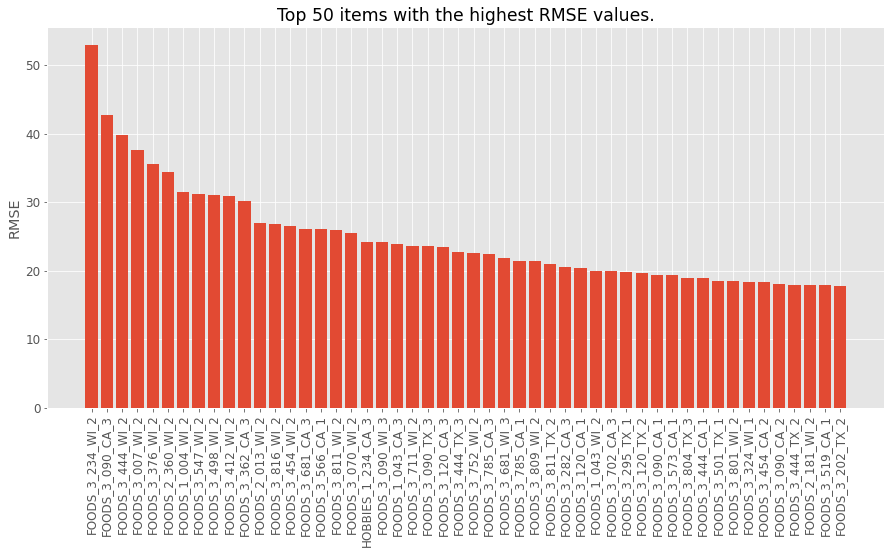
\includegraphics[width=0.95\textwidth]{figures/results/ann_worst.png}}
    \caption{Top 50 items with the highest RMSE for the MLP model.}
    \label{fig:ann_worst}
\end{figure}

\begin{figure}
    \centering
    \fbox{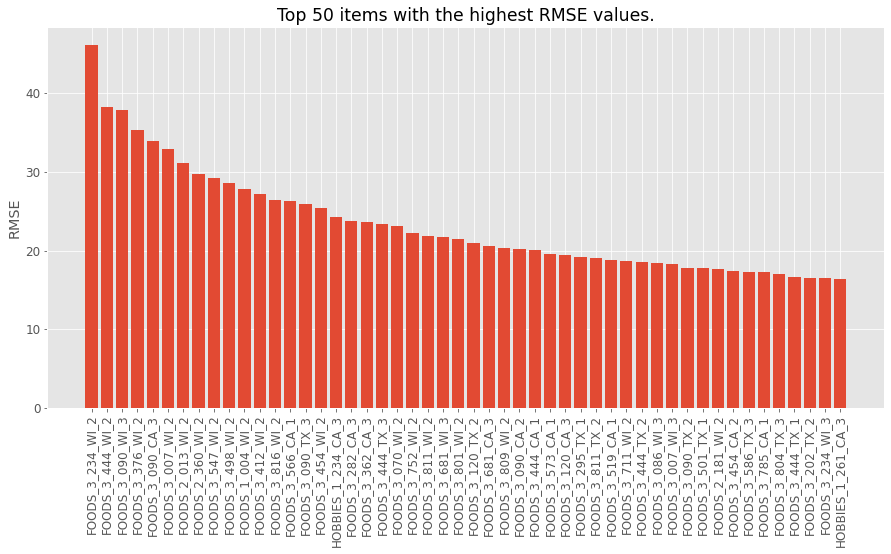
\includegraphics[width=0.95\textwidth]{figures/results/lgbm_worst.png}}
    \caption{Top 50 items with the highest RMSE for the LGBM model.}
    \label{fig:lgbm_worst}
\end{figure}

\begin{figure}
    \centering
    \fbox{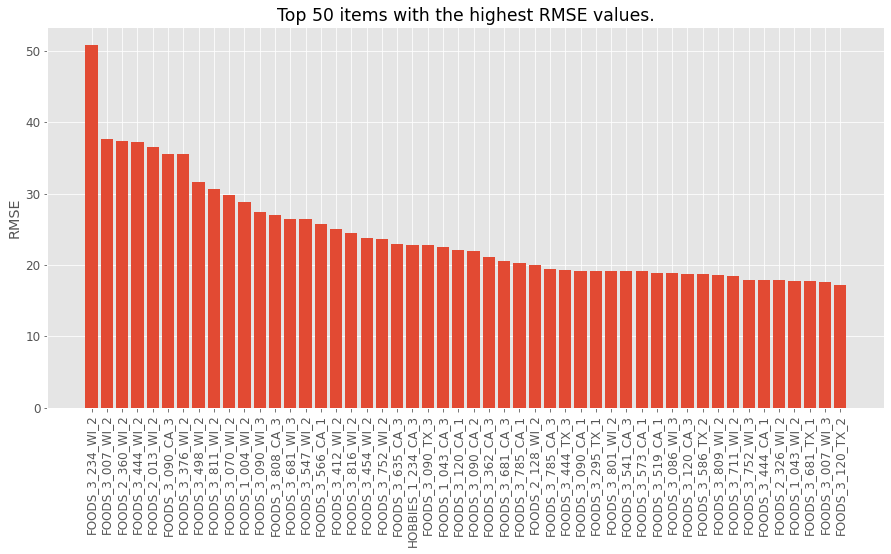
\includegraphics[width=0.95\textwidth]{figures/results/hyb_worst.png}}
    \caption{Top 50 items with the highest RMSE for the LSTM-LGBM hybrid model.}
    \label{fig:hyb_worst}
\end{figure}

\end{appendices}

\bibliographystyle{ieeetr}
\bibliography{references}

\end{document}
